\documentclass[journal]{IEEEtran}

\usepackage{amsmath,cite,graphicx}

\begin{document}

\title{The Constant-Q Transform Spectral Envelope Coefficients: A Timbre Feature Designed for Music}

\maketitle

\section{Scope}

\IEEEPARstart{T}{imbre} is the attribute of sound which makes, for example, two musical instruments playing the same note sound different. It is typically associated with the spectral (but also the temporal) envelope and assumed to be independent from the pitch (but also the loudness) of the sound \cite{moore2004}. In this article, we will show how to design a simple but functional pitch-independent timbre feature which is well adapted to musical data, by deriving it from the constant-Q transform (CQT), a log-frequency transform which matches the equal-tempered musical scale \cite{brown1991, brown1992}. We will show how to decompose the CQT spectrum into an energy-normalized pitch component and a pitch-independent spectral envelope, the latter from which we will extract a number of timbral coefficients. We will then evaluate the discriminative power of these \textit{CQT spectral envelope coefficients (CQT-SEC)} on the NSynth dataset \cite{engel2017}, a large-scale dataset of musical notes which is publicly available, comparing them with the mel-frequency cepstral coefficients (MFCCs) \cite{mermelstein1976}, features originally designed for speech recognition but commonly used to characterize timbre in music. 


\section{Relevance}

A timbre feature which is well adapted to musical data, pitch-independent, and with high discriminative power can find uses in a number of applications, such as similarity detection, sound recognition, and audio classification, in particular, of musical instruments. Additionally, the ability to decompose the spectrum of a sound (here, the CQT spectrum) into a pitch-independent spectral envelope and an energy-normalized pitch component can be useful for analysis, transformation, and resynthesis of music signals. The energy-normalized pitch component can also potentially be used for tasks such as pitch identification and melody extraction.


\section{Prerequisites}

Basic knowledge of audio signal processing and some knowledge of music information retrieval (MIR) \cite{mueller2007} are required to understand this article, in particular, concepts such as the Fourier transform (FT), convolution, spectral envelope, pitch, CQT, and MFCCs. More information about the CQT can also be found in \cite{brown1991, brown1992}.


\section{Problem Statement}

The multidimensional nature of timbre makes it an attribute that is tricky to quantify in terms of one simple characteristic feature \cite{grey1977}. While it is assumed to be independent from pitch and loudness, it is not really feasible to fully disentangle timbre from those qualities, as timbre is inherently dependent on the spectral content of the sound, which is also defined by its pitch and loudness \cite{moore2004}. Researchers in MIR proposed a number of descriptors to characterize one or more aspects of timbre \cite{peeters2011}, but they mostly resort to using the MFCCs when they need one simple timbre feature \cite{mueller2007}. While the MFCCs were shown to be practical in some MIR tasks, they were initially designed for speech processing applications \cite{mermelstein1976} and are not necessarily well adapted to musical data. In particular, they are derived through an old process which makes use of the mel scale, a perceptual scale experimentally designed 85 years ago to approximate the human auditory system's response \cite{stevens1937}. More recently, a number of data-driven approaches attempted to learn some timbral representations from musical data, but typically in terms of implicit embeddings which are tied to specific trained models \cite{engel2017, pons2017, hung2019, luo2019, lee2020} and not necessarily as explicit and interpretable features such as the MFCCs, which are still usually preferred as the go-to feature to characterize timbre by MIR practitioners.


\section{Solution}

We hereby present the CQT-SECs, a novel timbre feature which is well adapted to musical data, pitch-independent, simple to compute, interpretable, and functional. We will show how to derive it from the CQT, a frequency transform with a logarithmic resolution which matches the notes of the equal temperament, a tuning system typically used in Western music \cite{brown1991, brown1992}. We will first show how to decompose the CQT spectrum into a pitch-independent spectral envelope and an energy-normalized pitch component, and then extract a number of timbral coefficients from the spectral envelope. 

\subsection{Deconvolution of the CQT}

We start with the assumption that a log spectrum $S$, in particular, the CQT spectrum, can be represented as the convolution between a pitch-independent spectral envelope $E$ (which mostly contains the timbre information) and an energy-normalized pitch component $P$ (which mostly contains the pitch information), as shown in Equation \ref{eq:assumption}, where $*$ represents the convolution operation. 
\begin{equation}
\label{eq:assumption}
S = E * P
\end{equation}
This convolution process can be thought of as a source-filter model \cite{fant1970} which is here not applied in the time domain but in the frequency domain, with the source and the filter being the pitch component and the envelope, respectively.

\emph{Observation 1: A pitch change in the audio translates to a linear shift in the log spectrum \cite{brown1991, brown1992}.}

Assuming that pitch and timbre are independent, this implies that the same musical object at different pitches would have a similar envelope but a shifted pitch component (while two different musical objects at the same pitch would have different envelopes but a similar pitch component). This is summarized in Equation \ref{eq:observation1}, where $S$, $E$, $P$ and $S'$, $E'$, $P'$ represent the log spectrum, envelope, and pitch component for a musical object and for a pitch-shifted version of the same musical object, respectively.
\begin{equation}
\label{eq:observation1}
\begin{split}
& \begin{cases}
S = E * P \\
S' = E' * P' \\
\end{cases} \\
& \Rightarrow E \approx E'
\end{split}
\end{equation}

\emph{Observation 2: the FT of the convolution between two functions is equal to the pointwise product between the FTs of the two functions, a property known as the convolution theorem \cite{proakis1995}.}

This implies that the FT of the log spectrum is equal to the pointwise product between the FT of the envelope and the FT of the pitch component. Given the first observation, this further implies that the FT of the envelope for a musical object and for a pitch-shifted version of it would be equal. This is summarized in Equation \ref{eq:observation2}, where $\mathcal{F}(.)$ represents the FT function and $\cdot$ the pointwise product.
\begin{equation}
\label{eq:observation2}
\begin{split}
& \begin{cases}
\mathcal{F}(S) = \mathcal{F}(E * P) = \mathcal{F}(E) \cdot \mathcal{F}(P) \\
\mathcal{F}(S') = \mathcal{F}(E' * P') = \mathcal{F}(E') \cdot \mathcal{F}(P') \\
\end{cases} \\
& \Rightarrow \mathcal{F}(E) \approx \mathcal{F}(E')
\end{split}
\end{equation}

\emph{Observation 3: The magnitude FT is shift-invariant \cite{proakis1995}.}

This implies that the magnitude of the FT of the log spectrum for a musical object and for a pitch-shifted version of it would be equal. This is summarized in Equation \ref{eq:observation3}, where $|.|$ and $Arg(.)$ represent the modulus and argument, respectively, for a complex array, and $j$, the imaginary unit.
\begin{equation}
\label{eq:observation3}
\begin{split}
& \begin{cases}
\mathcal{F}(S) = |\mathcal{F}(S)| \cdot e^{j Arg(\mathcal{F}(S))} \\
\mathcal{F}(S') = |\mathcal{F}(S')| \cdot e^{j Arg(\mathcal{F}(S'))} \\
\end{cases} \\
& \Rightarrow |\mathcal{F}(S)| \approx |\mathcal{F}(S')|
\end{split}
\end{equation}

Given the previous observations, we can therefore conclude that the FT of the envelope could be approximated by the magnitude FT of the log spectrum, while the FT of the pitch component could be approximated by the phase component. This finally gives us the estimates for the envelope and the pitch component, after taking their inverse FTs, as shown in Equation \ref{eq:conclusion}, where $\mathcal{F}^{-1}(.)$ represents the inverse FT function.
\begin{equation}
\label{eq:conclusion}
\begin{split}
& \Rightarrow 
\begin{cases}
\mathcal{F}(E) \approx |\mathcal{F}(S)| \\
\mathcal{F}(P) \approx e^{j Arg(\mathcal{F}(S))} \\
\end{cases} \\
& \Rightarrow
\begin{cases}
E \approx \mathcal{F}^{-1}(|\mathcal{F}(S)|) \\
P \approx \mathcal{F}^{-1}(e^{j Arg(\mathcal{F}(S))}) \\
\end{cases}
\end{split}
\end{equation}

Figure \ref{fig:deconvolution} shows an example of deconvolution of a CQT spectrogram into its envelope and pitch component. The CQT spectogram was computed from an audio signal created by concatenating 12 4-second notes of an acoustic bass playing from C1 (32.70 Hz) to B1 (61.74 Hz) in ascending pitch. The notes come from the NSynth dataset \cite{engel2017} and correspond to instrument id \texttt{bass\_acoustic\_000}, MIDI numbers \texttt{024} to \texttt{035}, and velocity number \texttt{075}. The CQT spectrogram was computed using librosa \cite{mcfee2015, schoerkhuber2010}, with a sampling rate of 16 kHz, a hop length of 512 samples, a minimum frequency of 32.70 Hz (corresponding to C1), 95 frequency bins, and 12 bins per octave. As we can see, the envelope looks as if the CQT spectrogram has been normalized in pitch, with all the notes being brought down to the lowest frequency (corresponding to C1); while the pitch component looks as if the CQT spectrogram has been stripped down from its energy, leaving mostly the fundamental frequencies of the notes. Note that in practice, we use a power CQT spectrogram (i.e., magnitude to the power of 2) and take the real part for the envelope and pitch component to ensure real values. We can also potentially post-process this deconvolution, for example, by zeroing the few negative values in the pitch component and using it to derive a refined  envelope from the log spectrum.

\begin{figure*}[htp]
    \centering
    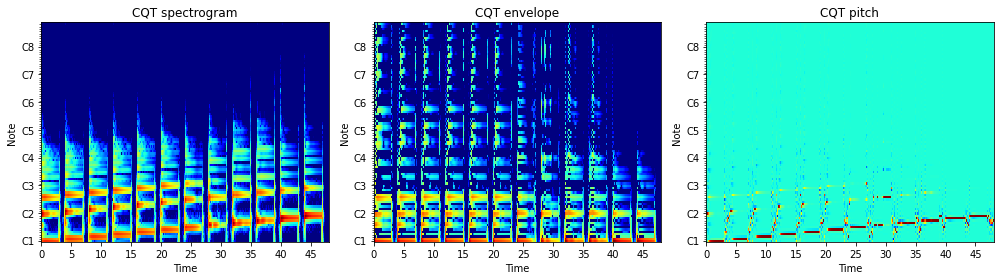
\includegraphics[width=\textwidth]{deconvolution.png}
    \caption{Deconvolution of the CQT spectrogram (left plot, shown in dB) of 12 acoustic bass notes playing from C1 to B1, into a pitch-independent spectral envelope (middle plot, shown in dB) and an energy-normalized pitch component (right plot, shown in $[0, 1]$).}
    \label{fig:deconvolution}
\end{figure*}

This deconvolution process can also be thought of as the normalization of the log spectrum by the magnitude of its FT (which here would correspond to the FT of the envelope) leading to a sharper log spectrum (which here would correspond to the pitch component), in the manner of the generalized cross-correlation phase transform (GCC-PHAT) method which aims at normalizing a cross-correlation function by its magnitude spectrum to sharpen the cross-correlation peaks \cite{knapp1976}.


\subsection{Extraction of the spectral envelope coefficients}

The envelope resulting from the deconvolution of the CQT spectrum can be thought of as a pitch-normalized CQT spectrum where the spectral content, in particular, the harmonics which represent most of the energy of the musical instrument, has been essentially brought down to the same lowest note level. Given the octave resolution which was used when computing the CQT spectrum, i.e., the number of bins per octave, we can then easily infer the locations of those harmonics in the envelope \cite{brown1991, brown1992}. We can subsequently extract these harmonics or \textit{spectral envelope coefficients} from the envelope and thus obtain a compact and interpretable feature for characterizing the timbre of the musical instrument. Equation \ref{eq:extraction} shows how to derive the indices of the spectral envelope coefficients given $O_r$, the octave resolution, and $N_c$, the number of desired coefficients, and finally extract the CQT-SECs from the envelope $E$, with $\log_2(.)$ and $round(.)$ representing the binary logarithm and the round function, respectively.
\begin{equation}
\label{eq:extraction}
\begin{split}
\begin{cases}
i = round(O_r \log_2(k)) \\
\text{CQT-SEC}_k = E(i) \\
\end{cases}
\quad 1 \le k \le N_c
\end{split}
\end{equation}

Figure \ref{fig:extraction} shows an example of CQT-SECs (on the left plot). 20 coefficients were extracted from the envelope resulting from the deconvolution of the CQT spectrogram of the musical signal shown in Figure \ref{fig:deconvolution}. These coefficients essentially correspond to the harmonics of the musical instrument which contain most of its spectral energy and can therefore be a reasonable representation of its timbre. For comparison, we also show the MFCCs computed from the same musical signal (on the right plot). 20 coefficients were computed using librosa \cite{mcfee2015}, with a sampling rate of 16 kHz, a window length of 1024 samples, and hop length of 512 samples, matching the time resolution of the CQT-SECs so that both features have the same size in time and frequency. 

\begin{figure*}[htp]
    \centering
    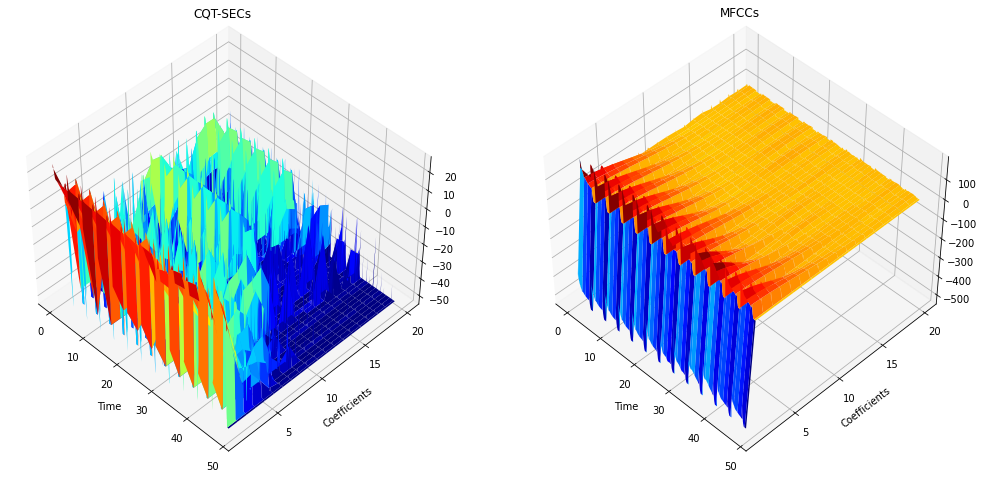
\includegraphics[width=\textwidth]{extraction.png}
    \caption{CQT-SECs extracted from the envelope obtained following the deconvolution of the CQT spectrogram shown in Figure \ref{fig:deconvolution} (left plot, shown in dB) and MFCCs computed from the same musical signal (right plot).}
    \label{fig:extraction}
\end{figure*}

We recall below how the MFCCs are commonly derived. First, a classic spectrogram is computed from the audio signal using the short-time Fourier transform (STFT) and the powers of the frequencies in each frame are then mapped onto the mel scale \cite{stevens1937} using triangular overlapping windows. This essentially produces a mel spectrogram. Then, the log of every mel frequency is taken, followed by the discrete cosine transform (DCT) of each frame. Finally, the MFCCs are selected as the lowest coefficients in the resulting spectrum, excluding the very first one (DC component). This process is meant to decouple the envelope from the pitch in the time domain, by extracting the slow-varying time components, which most likely correspond to the envelope and which will become the lowest coefficients, from the fast-varying time components, which most likely correspond to the pitch and which will become the highest coefficients \cite{mermelstein1976}. 


\section{A Computational Example}

We propose to measure the discriminative power of the CQT-SECs by evaluating them for a simple instrument similarity task on the NSynth dataset \cite{engel2017}, a large-scale and high-quality dataset of annotated musical notes which is publicly available\footnote{https://magenta.tensorflow.org/datasets/nsynth}. The NSynth dataset is composed of 305,979 musical notes which were generated from 1,006 instruments as 4-second, monophonic audio signals at a sampling rate of 16 kHz, with pitches ranging over all the note numbers of a standard MIDI piano (21-108) and with 5 different velocities (25, 50, 75, 100, and 127), whenever applicable. The instruments are organized into 11 families, namely, bass, brass, flute, guitar, keyboard, mallet, organ, reed, string, synth\_lead, and vocal, and 3 sources, namely, acoustic, electronic, and synthetic. We chose to evaluate the CQT-SECs on the notes with a velocity of 75 only, leading to a subset of 60,388 different notes for 945 different instruments.

We derived the CQT-SECs for all the notes in this subset, by first computing the CQT spectrogram using librosa, with a sampling rate of 16 kHz, a hop length of 512 samples, a minimum frequency of 32.70 Hz (corresponding to C1), 95 frequency bins, and 12 bins per octave, and then extracting 20 coefficients from the envelope resulting from the deconvolution of the CQT spectrogram, leading to CQT-SECs of size 20 (coefficients) by 126 (time frames). We used a power CQT spectrogram (i.e., magnitude to the power of 2) and took the real part for the envelope to ensure real values. For comparison, we also computed the MFCCs, using librosa, with a sampling rate of 16 kHz, a window length of 1024 samples, a hop length of 512 samples, and 20 coefficients, leading to MFCCs of same size as the CQT-SECs, i.e., 20 by 126.

We then computed the cosine similarity for every pair of CQT-SECs and every pair of MFCCs (without repetition), after flattening the features into vectors of length 2520 (20 times 126). We averaged these note similarities over every one of the 945 instruments, leading to similarity matrices of size 945 by 945, for both the CQT-SECs and the MFCCs. Figure \ref{fig:instrument_similarities} shows these instrument similarity matrices for the CQT-SECs and the MFCCs. As we can see, the similarities for the CQT-SECs have more variance, while the similarities for the MFCCs are mostly very high (close to 1) showing poor discriminative power between the different instruments. Figure \ref{fig:instrument_similarities2} additionally shows the self-similarities, i.e., the diagonal values in the similarity matrix (in green) and the error bars for the cross-similarities, i.e., the off-diagonal values in the similarity matrix (means in red and standard deviations in yellow) for every instrument, for the CQT-SECs and the MFCCs. As we can see, the self-similarities for the CQT-SECs are noticeably higher than the means of the cross-similarities for most of the instruments, and generally higher that the means plus standard deviations as well, showing good discriminative power, while the self-similarities and cross-similarities for the MFCCs are all very high (close to 1).

\begin{figure*}[htp]
    \centering
    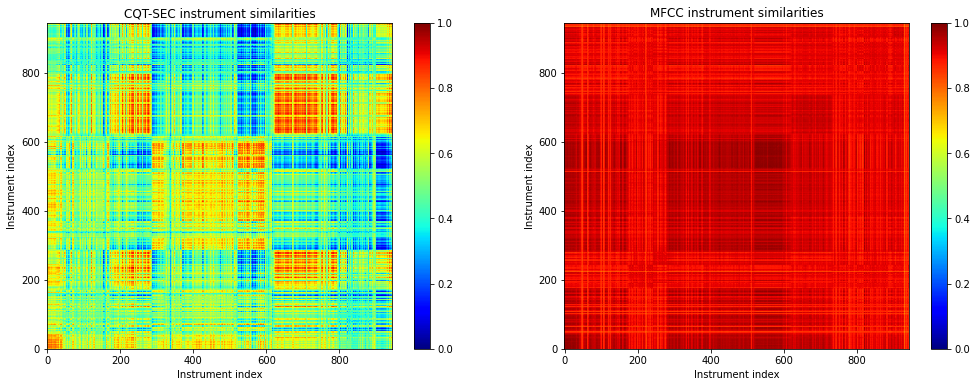
\includegraphics[width=\textwidth]{instrument_similarities.png}
    \caption{Similarity matrices computed for every pair of notes and averaged over every instrument of the NSynth subset, for the CQT-SECs (left plot) and the MFCCs (right plot).}
    \label{fig:instrument_similarities}
\end{figure*}

\begin{figure*}[htp]
    \centering
    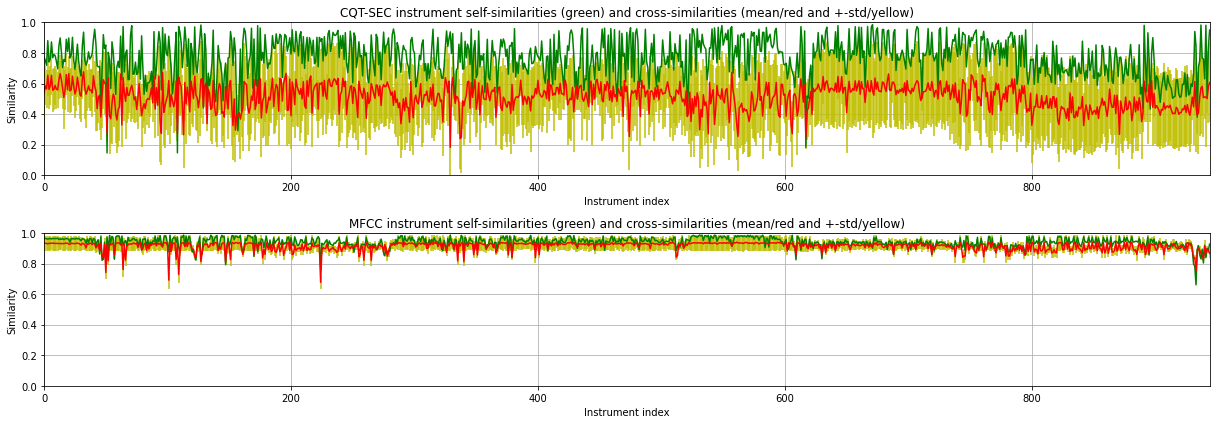
\includegraphics[width=\textwidth]{instrument_similarities2.png}
    \caption{Self-similarities and cross-similarities derived from the instrument similarity matrices shown in Figure \ref{fig:instrument_similarities}, for the CQT-SECs (top plot) and the MFCCs (bottom plot).}
    \label{fig:instrument_similarities2}
\end{figure*}

We also averaged the note similarities over every one of the 11 instrument families, leading to similarity matrices of size 11 by 11, for both the CQT-SECs and the MFCCs. Figure \ref{fig:family_similarities} shows these instrument family similarity matrices and figure \ref{fig:family_similarities2} additionally shows the self-similarities (in green) and the cross-similarities (means and standard deviations in red) for every instrument family, for the CQT-SECs and the MFCCs. As we can again see, the similarities for the CQT-SECs have more variance compared with the MFCCs, and their self-similarities are noticeably and mostly higher than the means plus standard deviations of their cross-similarities while the self-similarities and cross-similarities for the MFCCs are all very high and harder to tell apart. We can clearly see with the CQT-SECs, for example, that the organ family has high self-similarity, showing that most of the instruments and notes in that family are quite similar to each other in terms of timbre. We can also see that the organ family is somewhat similar to the brass, flute, and vocal families but quite different from the other families. On the other hand, the string family has fairly low self-similarity, showing that either the instruments or notes in that family differ substantially from each other, or the CQT-SECs were not able to properly capture the overall timbre for this family.

\begin{figure*}[htp]
    \centering
    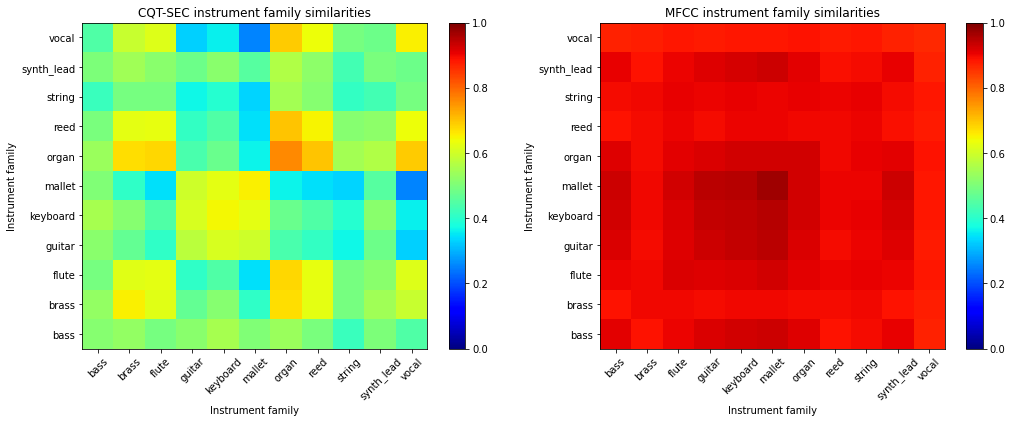
\includegraphics[width=\textwidth]{family_similarities.png}
    \caption{Similarity matrices computed for every pair of notes and averaged over every instrument family of the NSynth subset, for the CQT-SECs (left plot) and the MFCCs (right plot).}
    \label{fig:family_similarities}
\end{figure*}

\begin{figure*}[htp]
    \centering
    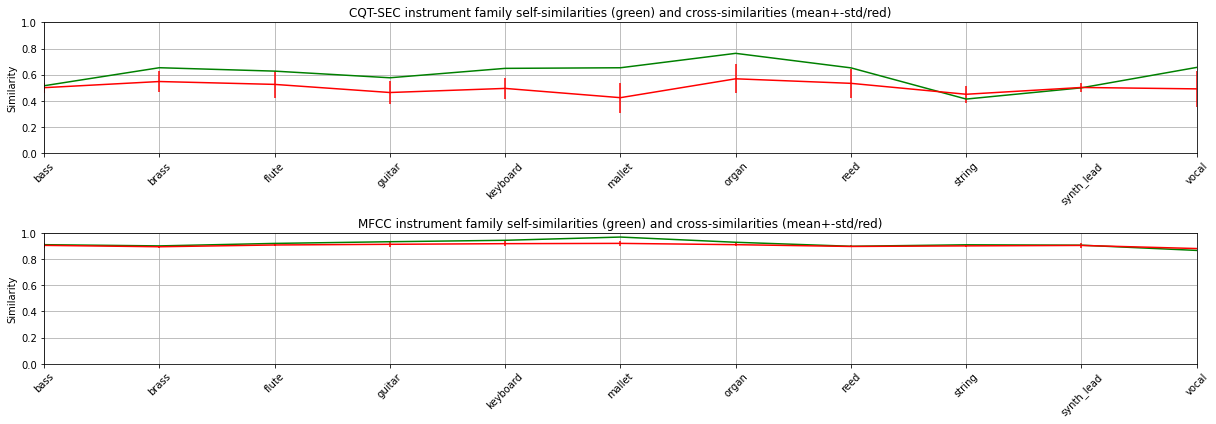
\includegraphics[width=\textwidth]{family_similarities2.png}
    \caption{Self-similarities and cross-similarities derived from the instrument family similarity matrices shown in Figure \ref{fig:family_similarities}, for the CQT-SECs (top plot) and the MFCCs (bottom plot).}
    \label{fig:family_similarities2}
\end{figure*}


\section{What We Have Learned}

We have shown that we can design a simple but functional pitch-independent timbre feature which is well-adapted to musical data by decomposing the CQT spectrum into a pitch-independent spectral envelope and an energy-normalized pitch component, and extracting a number of coefficients from the spectral envelope. These CQT-SECs provide a compact and interpretable feature for characterizing the timbre of a musical instrument, showing higher variance in terms of similarities on a simple instrument similarity task, compared with the MFCCs which are commonly used by MIR practitioners to characterize timbre in music. For the interested reader, we provide a Python implementation of the CQT-SEC online with some examples\footnote{https://github.com/zafarrafii/CQT-SEC-Python}.


\section{Author}

\textit{\textbf{Zafar Rafii}} (zafarrafii@gmail.com) received a PhD in Electrical Engineering and Computer Science from Northwestern University in 2014, and an MS in Electrical Engineering from both Ecole Nationale Superieure de l’Electronique et de ses Applications in France and Illinois Institute of Technology in the US in 2006. He is currently a research engineer manager at Gracenote in the US. He also worked as a research engineer at Audionamix in France. His research interests are centered on audio analysis, somewhere between signal processing, machine learning, and cognitive science, with a predilection for source separation and audio identification.

\bibliographystyle{IEEEtran}
\bibliography{bibliography.bib}

\end{document}
